% !TEX program = pdflatex
\documentclass{article}
% \input{preamble/preamble}
% \input{preamble/preamble_math}
\usepackage{url} 

\begin{document}

\title{\textbf{ML \& Climate | Final Report}}
\date{\today}
\author{Kent Liu, William Das}

\maketitle

\begin{abstract}
    Wildfires are a pressing environmental challenge, particularly in regions with complex topography and flammable vegetation, such as parts of the United States. This project proposes to harness topographic and environmental data from \textbf{LANDFIRE} alongside detailed wildfire event data—modeled after the \textbf{FIRED} curated data (linked below)—to predict wildfire spread rates and enhance simulation capabilities. Focusing on a U.S. region like California, this project aims to develop predictive models that can forecast daily fire spread rates and directions based on topographic and other meteorological features.

\end{abstract}

\section{Background}
Over the years, fire activity is increasing globally and warming temperatures and aridity are driving patterns of fire activities especially on the Western United States. \cite{https://doi.org/10.1111/j.1365-2699.2011.02595.x} While fire plays an important role in many natural processes such as nutrient cycling and habitat creation, unwarranted fires can be more detrimental than beneficial. They can hinder such natural processes and even put human lives at danger. Between 1990 and 2024, despite a 10 percent decrease in number of ignitions in the US, the annual area burned has increased by nearly 60 percent. \cite{wibbenmeyer2021wildfires}

To better understand and anticipate wildfire behavior, researchers now integrate high-resolution spatial datasets with historical fire event records. For instance, the \textbf{LANDFIRE} program \cite{landfire} offers over 20 national geospatial layers for the contiguous United States and U.S. insular areas, including elevation, slope, aspect, vegetation types, fuel models, and disturbance history. These layers provide essential environmental context that helps characterize landscape susceptibility to fire.

In addition, the \textbf{FIRED} datasets provide event-level and daily summaries of wildfires across the U.S., including key metrics such as ignition dates, total area burned, and daily spread rates. The existing \textbf{FIRED CONUS} dataset \cite{firedpy} specifically covers the contiguous U.S. from 2001 to 2019 and offers polygon-based fire perimeters with daily burn progression derived from MODIS satellite observations.

By integrating LANDFIRE’s environmental data with FIRED CONUS’s fire-specific data, we can construct robust machine learning models to predict fire dynamics such as daily spread rates (e.g., km\textsuperscript{2}/day), total spatial extent, or severity. This approach enables both retrospective analysis and predictive modeling of wildfire behavior. Furthermore, we extend our analysis to incorporate real-time fire incident data from 2025 \cite{calfire2025}, allowing us to evaluate model performance on recent and ongoing wildfire events in California and beyond.


\section{Exploratory Data Analysis}

\subsection{Basic Data}

We start with some analysis of the data. A good place to start is to look at the frequency of fires per year and the corresponding areas burned. The data for these corresponding categories appear to be highly correlated with oscillations between the years with peaks around 2004 and 2015.

\begin{figure}[htbp]
    \centering
    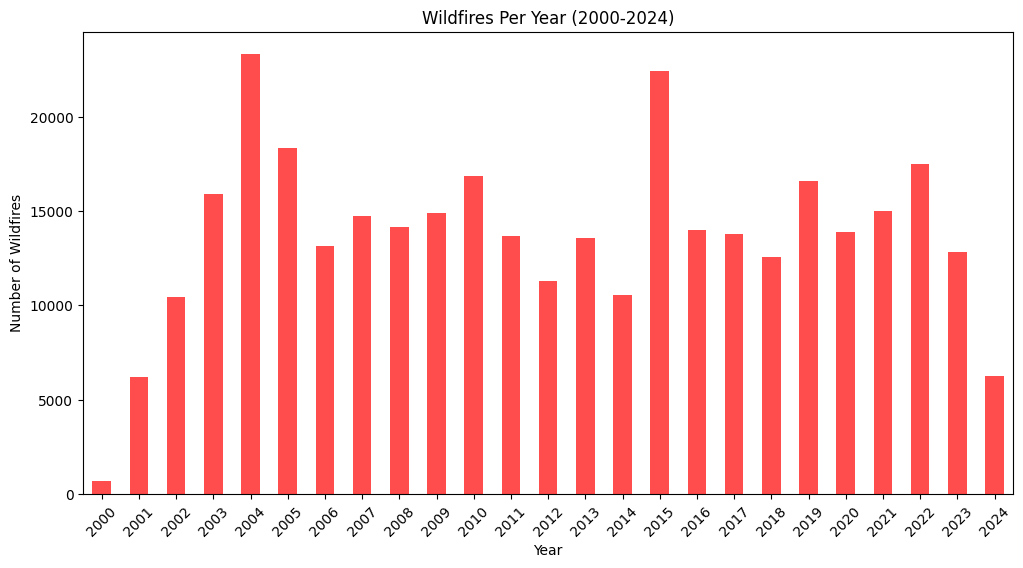
\includegraphics[width=0.8\textwidth]{img/fire_frequency.png}
    \caption{Plot for frequencies of wildfires per year from 2000-2024.}
    \label{fig:fire_frequency}
\end{figure}

\begin{figure}[htbp]
    \centering
    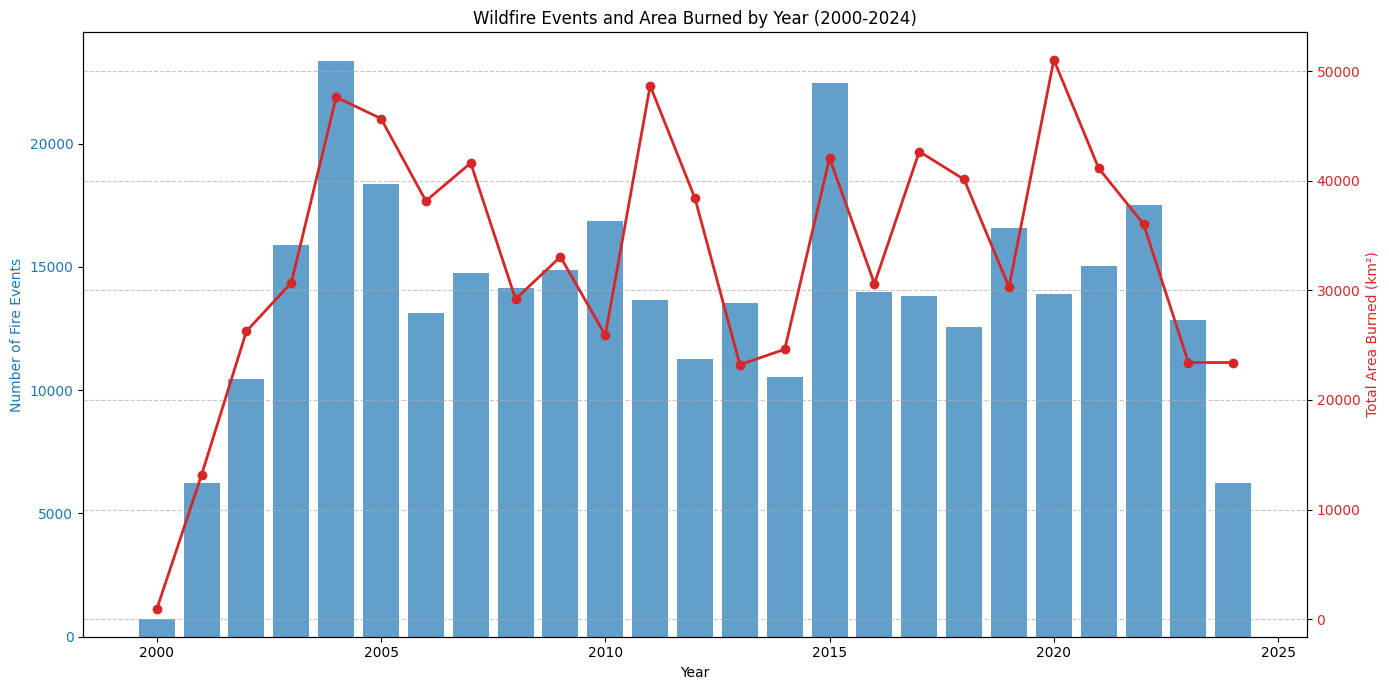
\includegraphics[width=0.8\textwidth]{img/fire_area.png}
    \caption{Plot for area burned by wildfires per year from 2000-2024.}
    \label{fig:fire_area}
\end{figure}


\subsection{Vegetation and Biome Data}
Vegetation and Biome plays a crucial role in wildfire ignition and spread. Drier and warmer areas tend to be more prone to fires starting. Patches and streaks of dead vegetation can catalyze the spread of such fires. From our analysis, Figure 3 shows that the Interior Alaska-Yukon lowland taiga leads with the largest burned area (approximately $68000 \text{ km}^2$), indicating that boreal forest ecosystems are particularly fire-prone. The Mississippi lowland forests and Flint Hills tall grasslands also exhibit high fire activity, which challenges the common notion that wildfires are confined to the western U.S.

Figure 4 shows the Ecological Diversity of Affected Regions. The top 10 includes forests, grasslands, shrub steppes, and wetland regions (Everglades)—showing wildfires impact a diverse range of ecosystems, suggesting that ecoregion-specific models might be necessary for accurate wildfire spread predictions. We can also gain some insight into geographic spread from this. Burned areas are spread across the country: from the Southeast (Mississippi, Everglades) to the West (Great Basin, Snake-Columbia) and North (Alaska), emphasizing that wildfire prediction efforts must be geographically comprehensive.



\begin{figure}[htbp]
    \centering
    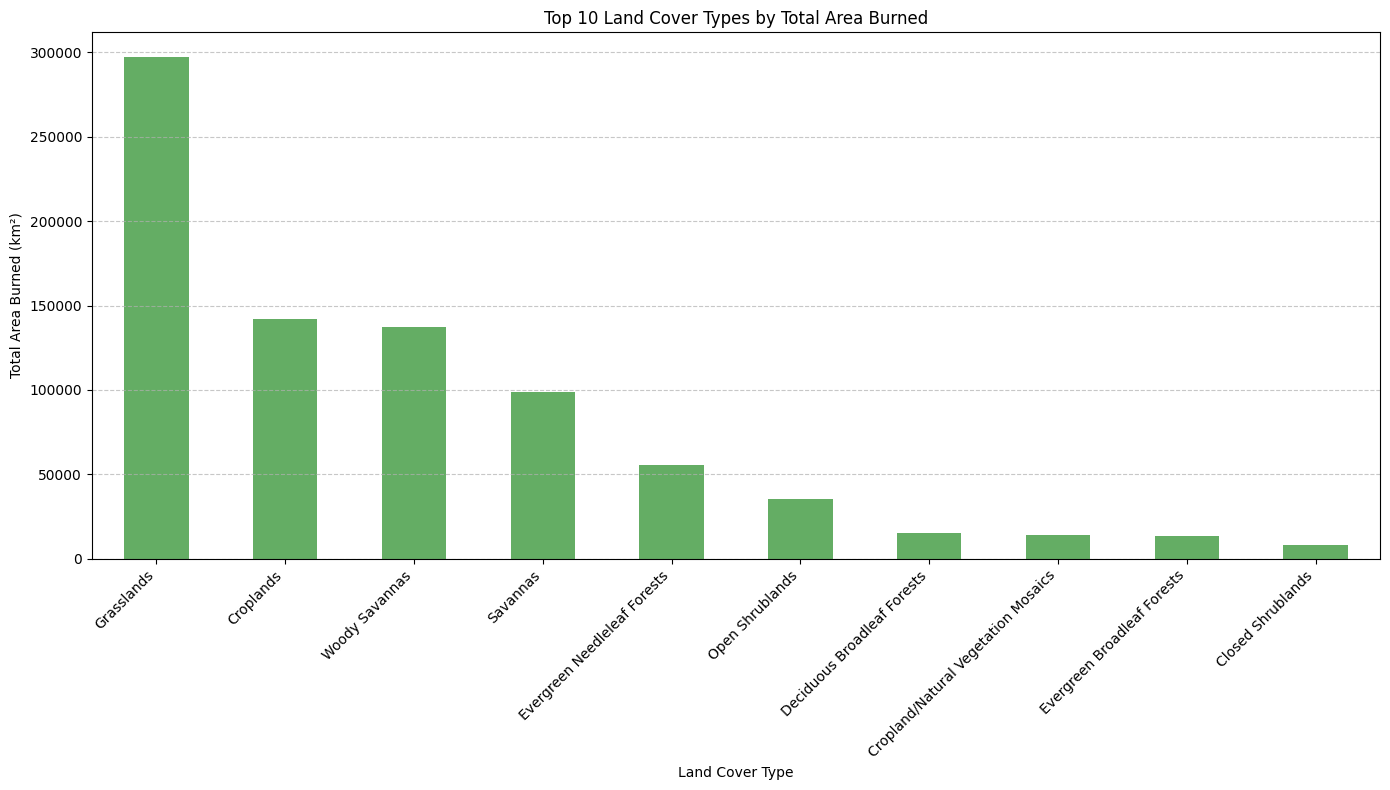
\includegraphics[width=0.8\textwidth]{img/land_cover.png}
    \caption{Plot for total area burned by land cover type from 2000-2024.}
    \label{fig:land_cover}
\end{figure}

\begin{figure}[htbp]
    \centering
    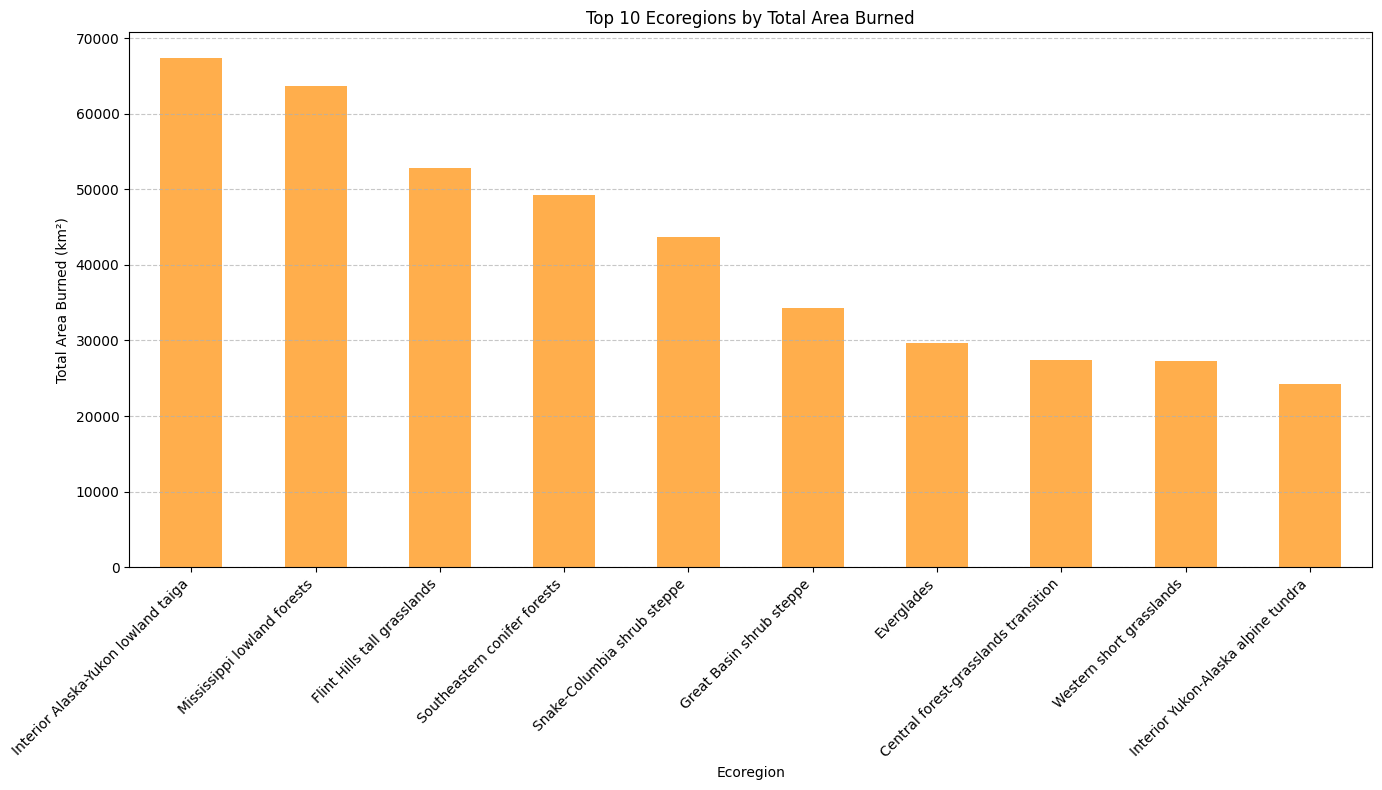
\includegraphics[width=0.8\textwidth]{img/ecoregions.png}
    \caption{Plot for total area burned by ecoregion from 2000-2024.}
    \label{fig:ecoregions}
\end{figure}

\bibliographystyle{abbrv}
\bibliography{reference}

\end{document}
